%% For double-blind review submission, w/o CCS and ACM Reference (max submission space)
\documentclass[sigplan,review]{acmart}\settopmatter{printfolios=true,printccs=false,printacmref=false}
%% For double-blind review submission, w/ CCS and ACM Reference
%\documentclass[sigplan,review,anonymous]{acmart}\settopmatter{printfolios=true}
%% For single-blind review submission, w/o CCS and ACM Reference (max submission space)
%\documentclass[sigplan,review]{acmart}\settopmatter{printfolios=true,printccs=false,printacmref=false}
%% For single-blind review submission, w/ CCS and ACM Reference
%\documentclass[sigplan,review]{acmart}\settopmatter{printfolios=true}
%% For final camera-ready submission, w/ required CCS and ACM Reference
%\documentclass[sigplan]{acmart}\settopmatter{}


%% Conference information
%% Supplied to authors by publisher for camera-ready submission;
%% use defaults for review submission.
\acmConference[FTfJP'19]{Workshop on on Formal Techniques for Java-like Programs}{July 15--19, 2019}{London, United Kingdom}
\acmYear{2019}
\acmISBN{} % \acmISBN{978-x-xxxx-xxxx-x/YY/MM}
\acmDOI{} % \acmDOI{10.1145/nnnnnnn.nnnnnnn}
\startPage{1}

%% Copyright information
%% Supplied to authors (based on authors' rights management selection;
%% see authors.acm.org) by publisher for camera-ready submission;
%% use 'none' for review submission.
\setcopyright{none}
%\setcopyright{acmcopyright}
%\setcopyright{acmlicensed}
%\setcopyright{rightsretained}
%\copyrightyear{2018}           %% If different from \acmYear

%% Bibliography style
\bibliographystyle{ACM-Reference-Format}
%% Citation style
%\citestyle{acmauthoryear}  %% For author/year citations
%\citestyle{acmnumeric}     %% For numeric citations
%\setcitestyle{nosort}      %% With 'acmnumeric', to disable automatic
                            %% sorting of references within a single citation;
                            %% e.g., \cite{Smith99,Carpenter05,Baker12}
                            %% rendered as [14,5,2] rather than [2,5,14].
%\setcitesyle{nocompress}   %% With 'acmnumeric', to disable automatic
                            %% compression of sequential references within a
                            %% single citation;
                            %% e.g., \cite{Baker12,Baker14,Baker16}
                            %% rendered as [2,3,4] rather than [2-4].


%%%%%%%%%%%%%%%%%%%%%%%%%%%%%%%%%%%%%%%%%%%%%%%%%%%%%%%%%%%%%%%%%%%%%%
%% Note: Authors migrating a paper from traditional SIGPLAN
%% proceedings format to PACMPL format must update the
%% '\documentclass' and topmatter commands above; see
%% 'acmart-pacmpl-template.tex'.
%%%%%%%%%%%%%%%%%%%%%%%%%%%%%%%%%%%%%%%%%%%%%%%%%%%%%%%%%%%%%%%%%%%%%%


%% Some recommended packages.
\usepackage{booktabs}   %% For formal tables:
                        %% http://ctan.org/pkg/booktabs
\usepackage{subcaption} %% For complex figures with subfigures/subcaptions
                        %% http://ctan.org/pkg/subcaption


%% Pkgs
%% =============================================================================

%% %%%%%%%%%%%%%%%%%%%%%%%%%%%%%%%%%% Style

%\usepackage{url}
%\usepackage{hyperref}
\usepackage{xspace}

%% %%%%%%%%%%%%%%%%%%%%%%%%%%%%%%%%%% Math

\usepackage{mathpartir} % inference rules

%% %%%%%%%%%%%%%%%%%%%%%%%%%%%%%%%%%% Graphics

\usepackage{tikz}
\usetikzlibrary{fit,shapes, positioning}


%% Commands
%% =============================================================================

%% Text
%% *********************************************************

\newcommand{\defemph}[1]{\textbf{#1}}

\newcommand{\jlcode}[1]{\texttt{\small#1}}
\newcommand{\jltype}[1]{\texttt{\small#1}}

\newcommand{\figref}[1]{Fig.~\ref{#1}}
\newcommand{\secref}[1]{Sec.~\ref{#1}}

\newcommand{\citemock}{\cite{bib:mock}\xspace}

%% %%%%%%%%%%%%%%%%%%%%%%%%%%%%%%%%%% BetaJulia

\newcommand{\BetaJulia}{\textsc{MiniJl}\xspace}
\newcommand{\BetaJuliaSub}{\textsc{JNomSub}\xspace}


%% General Math/PL
%% *********************************************************

%: \Alt                 -> |
\newcommand{\Alt}{~\vert~}

%% BetaJulia
%% *********************************************************

%% %%%%%%%%%%%%%%%%%%%%%%%%%%%%%%%%%% Style

%: type name (like Int)
\newcommand{\tyname}[1]{\ensuremath{\mathsf{#1}}}

%% %%%%%%%%%%%%%%%%%%%%%%%%%%%%%%%%%% Metavariables

%: \ty                  -> τ
\newcommand{\ty}{\ensuremath{\tau}\xspace}
%: \vty                 -> v
\newcommand{\vty}{\ensuremath{v}\xspace}

\newcommand{\cname}{\ensuremath{\mathit{cname}}\xspace}
\newcommand{\aname}{\ensuremath{\mathit{aname}}\xspace}

\newcommand{\Type}{\textsc{Type}\xspace}
\newcommand{\VType}{\textsc{ValType}\xspace}
\newcommand{\PVType}{\ensuremath{\mathcal{P}(\VType)}}

\newcommand{\NomH}{\textrm{NomHrc}\xspace}
\newcommand{\NomHClosure}{\textrm{NomHrc*}\xspace}


%% %%%%%%%%%%%%%%%%%%%%%%%%%%%%%%%%%% Type Constructors

%: \typair{t1}{t2}      -> t1 × t2
\newcommand{\typair}[2]{\ensuremath{#1 \times #2}}

%: \tyunion{t1}{t2}     -> t1 ∪ t2
\newcommand{\tyunion}[2]{\ensuremath{#1 \cup #2}}

%% %%%%%%%%%%%%%%%%%%%%%%%%%%%%%%%%%% Type Examples

\newcommand{\tysigned}{\tyname{Signed}\xspace}
\newcommand{\tyintsf}{\tyname{Int64}\xspace}
\newcommand{\tyinttt}{\tyname{Int32}\xspace}
\newcommand{\tyintst}{\tyname{Int16}\xspace}

\newcommand{\tynum}{\tyname{Num}\xspace}
\newcommand{\tyreal}{\tyname{Real}\xspace}
\newcommand{\tyint}{\tyname{Int}\xspace}
\newcommand{\tyflt}{\tyname{Flt}\xspace}
\newcommand{\tycmplx}{\tyname{Cmplx}\xspace}
\newcommand{\tystr}{\tyname{Str}\xspace}

%% %%%%%%%%%%%%%%%%%%%%%%%%%%%%%%%%%% Nominal Hierarchy

\newcommand{\bjdeclsub}[2]{\ensuremath{#1 \rhd #2}}
\newcommand{\bjnomsub}[2]{\ensuremath{#1\,{\rhd^*} #2}}

%% %%%%%%%%%%%%%%%%%%%%%%%%%%%%%%%%%% Interpretation

\newcommand{\interpty}[1]{\ensuremath{\llbracket #1 \rrbracket}}



\begin{document}

%% Title information
\title[Short Title]{Syntactic Model of Semantic Subtyping \\
	for a Dynamic Language with Nominal Typing}
                                        %% [Short Title] is optional;
                                        %% when present, will be used in
                                        %% header instead of Full Title.
\titlenote{with title note}             %% \titlenote is optional;
                                        %% can be repeated if necessary;
                                        %% contents suppressed with 'anonymous'
\subtitle{Subtyping of Nominal Types, Pairs, and Unions}
                                        %% \subtitle is optional
\subtitlenote{with subtitle note}       %% \subtitlenote is optional;
                                        %% can be repeated if necessary;
                                        %% contents suppressed with 'anonymous'


%% Author information
%% Contents and number of authors suppressed with 'anonymous'.
%% Each author should be introduced by \author, followed by
%% \authornote (optional), \orcid (optional), \affiliation, and
%% \email.
%% An author may have multiple affiliations and/or emails; repeat the
%% appropriate command.
%% Many elements are not rendered, but should be provided for metadata
%% extraction tools.

%% Author with single affiliation.
\author{Julia Belyakova}
%\authornote{with author1 note}          %% \authornote is optional;
                                        %% can be repeated if necessary
\orcid{nnnn-nnnn-nnnn-nnnn}             %% \orcid is optional
\affiliation{
%  \position{Position1}
%  \department{Khoury College of Computer Sciences}              %% \department is recommended
  \institution{Northeastern University}            %% \institution is required
%  \streetaddress{Street1 Address1}
%  \city{Boston}
%  \state{MA}
%  \postcode{Post-Code1}
%  \country{USA}                    %% \country is recommended
}
\email{belyakova.y@northeastern.edu}          %% \email is recommended

%%% Author with two affiliations and emails.
%\author{First2 Last2}
%\authornote{with author2 note}          %% \authornote is optional;
%                                        %% can be repeated if necessary
%\orcid{nnnn-nnnn-nnnn-nnnn}             %% \orcid is optional
%\affiliation{
%  \position{Position2a}
%  \department{Department2a}             %% \department is recommended
%  \institution{Institution2a}           %% \institution is required
%  \streetaddress{Street2a Address2a}
%  \city{City2a}
%  \state{State2a}
%  \postcode{Post-Code2a}
%  \country{Country2a}                   %% \country is recommended
%}
%\email{first2.last2@inst2a.com}         %% \email is recommended
%\affiliation{
%  \position{Position2b}
%  \department{Department2b}             %% \department is recommended
%  \institution{Institution2b}           %% \institution is required
%  \streetaddress{Street3b Address2b}
%  \city{City2b}
%  \state{State2b}
%  \postcode{Post-Code2b}
%  \country{Country2b}                   %% \country is recommended
%}
%\email{first2.last2@inst2b.org}         %% \email is recommended


%% Abstract
%% Note: \begin{abstract}...\end{abstract} environment must come
%% before \maketitle command
\begin{abstract}
Text of abstract \ldots.
\end{abstract}


%% 2012 ACM Computing Classification System (CSS) concepts
%% Generate at 'http://dl.acm.org/ccs/ccs.cfm'.
\begin{CCSXML}
<ccs2012>
<concept>
<concept_id>10011007.10011006.10011008</concept_id>
<concept_desc>Software and its engineering~General programming languages</concept_desc>
<concept_significance>500</concept_significance>
</concept>
<concept>
<concept_id>10003456.10003457.10003521.10003525</concept_id>
<concept_desc>Social and professional topics~History of programming languages</concept_desc>
<concept_significance>300</concept_significance>
</concept>
</ccs2012>
\end{CCSXML}

\ccsdesc[500]{Software and its engineering~General programming languages}
\ccsdesc[300]{Social and professional topics~History of programming languages}
%% End of generated code


%% Keywords
%% comma separated list
\keywords{keyword1, keyword2, keyword3}  %% \keywords are mandatory in final camera-ready submission


%% \maketitle
%% Note: \maketitle command must come after title commands, author
%% commands, abstract environment, Computing Classification System
%% environment and commands, and keywords command.
\maketitle


\section{Introduction}

Subtyping is utilized by many static type systems.
Informally, a subtyping relation \jltype{T $<:$ S} states that
a value of type~\jltype{T} can be safely used
in the context that expects a value of type~\jltype{S}.
For example, if class \jltype{Rectangle} is a subtype of class \jltype{Shape},
than a function with an argument of type \jltype{Shape}
can be called with an instance of \jltype{Rectangle}. 

Subtyping can also be used for run-time dispatch of function calls, 
in particular, \emph{multiple dynamic dispatch} 
(MDD)~\cite{bib:Chambers:1992:Cecil,bib:Clifton:2000:MultiJava}.
It allows a function to have several implementations 
for different types of arguments,
and the most suitable implementation for a particular call 
is picked dynamically, based on the run-time types of all arguments.
%and their subtyping relation to the function signatures.
For example, consider two implementations of addition,
\jlcode{+(Number, Number)} and \jlcode{+(String, String)},
and the call \jlcode{3+5}.
In this case, a language run-time should pick 
the implementation for numbers 
because \jltype{Int $<:$ Number} but \jltype{Int $\not{<:}$ String}.

It is often convenient to think of subtyping \jltype{T $<:$ S}
in terms of the set inclusion: ``the elements of~\jltype{T} are a subset
of the elements of~\jltype{S}''~\cite{bib:Pierce:2002:TAPL}.
This intuition is not always correct, but, in the case of
\emph{semantic subtyping}~\cite{bib:Hosoya:2003:XDuce,
  bib:Frisch:2008:sem-sub, bib:Ancona:2016:sem-sub-oo}, 
subtyping is defined exactly as the subset relation. % on values.
Namely, types are interpreted as sets
$\interpty{\ty} = \{\nu \Alt \vdash \nu : \ty \}$, 
and subtyping $\ty_1 <: \ty_2$ is defined as inclusion 
of the interpretations
$\interpty{\ty_1} \subseteq \interpty{\ty_2}$.

While the semantic definition of subtyping intertwines with 
a static typing relation,
subtyping is applicable in the context of 
\emph{dynamically} typed languages.
As mentioned before, subtyping can be used for multiple dynamic dispatch,
and MDD is rather widespread among dynamic languages
such as CLOS, Julia, Clojure.
Unlike statically typed languages, 
which conservatively prevent type errors with static checking,
dynamic languages detect type errors at run-time.
Namely, whenever an operator is restricted to certain kinds of values,
the language run-time checks the arguments of the operator before running it;
often, such a check amounts to checking the \emph{type tag} associated 
with the value argument.

A large number of dynamic languages provide support 
for object-oriented programming with classes, 
thus enabling user-defined hierarchies of nominal types.
%that can be used for dynamic dispatch.
Nominal types are the main source of type tags: 
any class that can be instantiated induces a tag (the name of the class) 
that is used to tag all the instances.
Abstract classes and interfaces, on the other hand, 
do not have instances, so do not induce tags.

In this paper, we are bridging the gap between \emph{semantic} subtyping 
and \emph{dynamically} typed languages with \emph{nominal} types.
Instead of directly interpreting types as sets of values,
we interpret them as sets of \emph{type tags} assuming 
each value is associated with a tag.
Our contributions are as follows:
\begin{enumerate}
  \item Tag-based semantic interpretation of types for a language
    with nominal types, tuples, and unions (\secref{sec:semsub}).
  \item Two syntactic definitions of subtyping, declarative and reductive,
    along with the Coq-mechanized proofs that the definitions are equivalent
    and coincide with the semantic interpretation (\secref{sec:synsub}). 	
  \item Proof of decidability of the reductive subtyping.
  \item Discussion of the implications of using semantic subtyping
    for multiple dynamic dispatch (\secref{sec:discussion}).
\end{enumerate}








\section{???}

We build the presentation around a small type language called \BetaJulia,
presented in~\figref{fig:bjsem-types}.
Types of \BetaJulia, denoted by $\ty \in \Type$, include pairs, unions, 
and nominal types in the spirit of Julia:
\cname denotes \emph{concrete} nominal types that correspond to type tags,
and \aname denotes \emph{abstract} nominal types.
In this terminology, \jltype{Int64} and \jltype{Signed} are
a concrete and abstract type, respectively.\footnote{Correspondence to Julia.}

\begin{figure}
	\[
	\begin{array}{rcl@{\qquad}l}
	\ty \in \Type & ::= & & \text{\emph{Types}}
	\\ &\Alt& \typair{\ty_1}{\ty_2}  & \text{covariant pair}
	\\ &\Alt& \tyunion{\ty_1}{\ty_2} & \text{untagged union}
	\\ &\Alt& \cname  & \text{concrete nominal type}
	\\ &\Alt& \aname  & \text{abstract nominal type}
	\\ \\
	\cname & \in &
	\multicolumn{2}{l}{\{ \tyint, \tyflt, \tycmplx, \tystr \}}
	\\ 
	\aname & \in & \multicolumn{2}{l}{\{ \tyreal, \tynum \}}
	\end{array}
	\]
	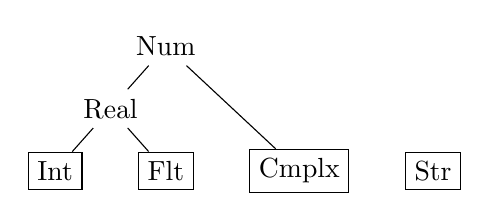
\begin{tikzpicture}[sibling distance=4em, level distance=2.25em,
	concrete/.style = {shape=rectangle, draw, align=center}]
	\node { Num }
	child { node { Real }
		child { node[concrete] { Int} }
		child { node[concrete] (NF) { Flt} } }
	child { node[concrete, right=2em of NF] (NC) {Cmplx} }
	;
	\node[concrete, right=2em of NC] {Str} ;
	\end{tikzpicture}
	\caption{\BetaJulia: type grammar and nominal hierarchy}
	\label{fig:bjsem-types}
\end{figure}

To simplify the development, we decided to work with particular 
nominal types and a hierarchy over them
(presented in~\figref{fig:bjsem-types} as a tree)
instead of a more abstract class table.
There are four concrete, leaf types (depicted in rectangles)
and two abstract types in the hierarchy. 
Formally, the hierarchy can be represented with a list of declarations
$\bjdeclsub{n_1}{n_2}$ read as ``$n_1$ is a declared subtype of $n_2$''
where $n ::= \cname \Alt \aname$.
In the case of \BetaJulia, the hierarchy is defined as follows:
\[
\NomH = [ \bjdeclsub{\tyreal}{\tynum}, 
\bjdeclsub{\tyint}{\tyreal}, \bjdeclsub{\tyflt}{\tyreal},
\bjdeclsub{\tycmplx}{\tynum} ].
\]
\TODO{requirements for hierarchy, like single parent, no cycles}

\subsection{Value Types}
%% -----------------------------------------------------------------------------

Not only concrete nominal types can be used as type tags
but also pair types. For example, \typair{\tyint}{\tyint}
or \typair{\tystr}{(\typair{\tyint}{\tyint})}.
Union types, on the other hand, cannot be type tags, 
as they potentially describe dissimilar values.
For instance, both integer and floating point values belong
to a union type \tyunion{\tyint}{\tyflt}.
Even type \tyunion{\tyint}{\tyint} is not a type tag, 
though it better be equivalent to a concrete type \tyint.

Types that can be used as type tags will be further referred to
as \defemph{value types}. 
Their formal definition is given in~\figref{fig:bjsem-value-types}:
value type $\vty \in \VType$ is either a concrete nominal type 
or a pair of value types. 
Note that $\VType \subset \Type$, i.e. each value type is a type.

\begin{figure}
	\[
	\begin{array}{rcl@{\qquad}l}
	\vty \in \VType & ::= & & \text{\emph{Value Types}}
	\\ &\Alt& \cname & \text{concrete nominal type}
	\\ &\Alt& \typair{\vty_1}{\vty_2} & \text{pair of value types}
	\end{array}
	\]
	\caption{Value types in \BetaJulia}
	\label{fig:bjsem-value-types}
\end{figure}


\subsection{Semantic Interpretation of Types}
%% -----------------------------------------------------------------------------

As mentioned earlier, the set of values represented by a value type \vty
is unambiguously characterized by~\vty itself
as long as each run-time value is tagged with a value type.
But what about an arbitrary type?

First, let us consider an abstract nominal type, e.g. \tynum. 
According to the nominal hierarchy, \tynum value 
is either a concrete complex number, or a real number, which, in turn,
is either a concrete integer or a floating point number.
Therefore, the set of values represented by \tynum 
is described by the set of value types $\{\tycmplx, \tyint, \tyflt\}$.

Next, pairs. Consider type \typair{\tystr}{\tyreal}:
each of its values is a pair of a string and a number. 
For example, \jlcode{("bread", 2)} and \jlcode{("milk", 2.75)} are such values, 
with type tags \typair{\tystr}{\tyint} and 
\typair{\tystr}{\tyflt}, respectively.

\begin{figure}
  \[
	\begin{array}{rcl}
	\interpty{\cdot}: \Type &\rightarrow& \PVType \\
	\interpty{\cname}  & = & \{\cname\} \\
	\interpty{\tyreal} & = & \{ \tyint, \tyflt \} \\
	\interpty{\tynum} & = & \{ \tyint, \tyflt, \tycmplx \} \\
	\interpty{\typair{\ty_1}{\ty_2}} & = & \{\typair{\vty_1}{\vty_2} 
	\Alt \vty_1 \in \interpty{\ty_1}, \vty_2 \in \interpty{\ty_2}\}\\
	\interpty{\tyunion{\ty_1}{\ty_2}} & = & 
	\interpty{\ty_1} \cup \interpty{\ty_2}
	\end{array}
  \]
%  	\interpty{\aname} & = & \{\cname\ \Alt \bjnomsub{\cname}{\aname} \} \\
%  (= \interpty{\tyreal} \cup \{\tycmplx\})
  \caption{Semantic Interpretation of \BetaJulia Types}
  \label{fig:bjsem-interpretation}
\end{figure}

Formally, the \emph{interpretation} of \BetaJulia types is defined
in~\figref{fig:bjsem-interpretation}.
Abstract types are interpreted according to the nominal hierarchy:
values of each abstract type are values of any of it value subtypes.
More generally, the interpretation of abstract types can be given in
then following way:
\[
\interpty{\aname} = \{\cname\ \Alt \bjnomsub{\cname}{\aname} \},
\]
where the relation $\bjnomsub{n_1}{n_2}$,
read ``$n_1$ is a nominal subtype of~$n_2$'',
is a transitive closure of $\bjdeclsub{n_1}{n_2}$:
\begin{mathpar}
	\inferrule*[right=]
	{ \bjdeclsub{n_1}{n_2} \in \NomH }
	{ \bjnomsub{n_1}{n_2} }
	
	\inferrule*[right=]
	{ \bjnomsub{n_1}{n_2} \\ \bjnomsub{n_2}{n_3} }
	{ \bjnomsub{n_1}{n_3} }.
\end{mathpar}
\TODO{Probably more on the semantic interpretation.}

Once we have the interpretation of types, we define \emph{semantic subtyping}
as the subset relation:
\[
\bjtruesemsub{\ty_1}{\ty_2} \quad \defsign \quad
\interpty{\ty_1} \subseteq \interpty{\ty_2}.
\]

%and the set of values represented by a type \ty can be characterized
%with the set of value types~$\vty_i$



%% Acknowledgments
\begin{acks}                            %% acks environment is optional
                                        %% contents suppressed with 'anonymous'
  %% Commands \grantsponsor{<sponsorID>}{<name>}{<url>} and
  %% \grantnum[<url>]{<sponsorID>}{<number>} should be used to
  %% acknowledge financial support and will be used by metadata
  %% extraction tools.
%  This material is based upon work supported by the
%  \grantsponsor{GS100000001}{National Science
%    Foundation}{http://dx.doi.org/10.13039/100000001} under Grant
%  No.~\grantnum{GS100000001}{nnnnnnn} and Grant
%  No.~\grantnum{GS100000001}{mmmmmmm}.  Any opinions, findings, and
%  conclusions or recommendations expressed in this material are those
%  of the author and do not necessarily reflect the views of the
%  National Science Foundation.
\end{acks}


%% Bibliography
\bibliography{bibfile}


%% Appendix
\appendix
\section{Appendix}

Text of appendix \ldots

\end{document}
